\chapter{Glossary \& Quick Reference}\label{ch:glossary}

\begin{nontechnical}
\textbf{This glossary is your quick-reference guide} to the terminology, acronyms, and key concepts used throughout this book.

\textbf{Structure:}
\begin{itemize}
\item \textbf{Acronyms A--Z}: Quick lookup of abbreviations
\item \textbf{Key Concepts}: Detailed explanations with equations and diagrams
\item \textbf{Cross-references}: Links to detailed chapter coverage
\end{itemize}

\textbf{Usage tip:} Use Ctrl+F (Cmd+F on Mac) to search for any term instantly.
\end{nontechnical}

\section{Overview}

This glossary serves as a comprehensive quick-reference guide for practitioners, students, and researchers in digital communications and signal processing. Each entry provides concise definitions with cross-references to detailed chapter coverage where applicable.

\begin{keyconcept}
\textbf{Understanding the notation:} Terms marked with {[}{[}Chapter-Name{]}{]} have dedicated chapters providing in-depth coverage. Mathematical symbols and equations use standard IEEE and ITU notation.
\end{keyconcept}

\section{Acronyms \& Abbreviations}

\subsection{A}\label{a}

\textbf{ACK} - Acknowledgment\\
\textbf{ADC} - Analog-to-Digital Converter\\
\textbf{AESA} - Active Electronically Scanned Array\\
\textbf{AFC} - Automatic Frequency Control\\
\textbf{AGC} - Automatic Gain Control\\
\textbf{AID} - Adaptive Impedance Demodulation (from
{[}{[}AID-Protocol-Case-Study{]}{]})\\
\textbf{AM} - Amplitude Modulation\\
\textbf{AMC} - {[}{[}Adaptive-Modulation-\&-Coding-(AMC){]}{]}\\
\textbf{AR} - Axial Ratio (polarization)\\
\textbf{ARQ} - Automatic Repeat Request\\
\textbf{ASK} - {[}{[}Amplitude-Shift-Keying-(ASK){]}{]}\\
\textbf{AWGN} - {[}{[}Additive-White-Gaussian-Noise-(AWGN){]}{]}

\subsection{B}\label{b}

\textbf{BCH} - Bose-Chaudhuri-Hocquenghem codes (see
{[}{[}Block-Codes-(Hamming,-BCH,-Reed-Solomon){]}{]})\\
\textbf{BER} - {[}{[}Bit-Error-Rate-(BER){]}{]}\\
\textbf{BPSK} - {[}{[}Binary-Phase-Shift-Keying-(BPSK){]}{]}

\subsection{C}\label{c}

\textbf{CDF} - Cumulative Distribution Function\\
\textbf{CFO} - Carrier Frequency Offset\\
\textbf{CQI} - Channel Quality Indicator\\
\textbf{CRC} - Cyclic Redundancy Check

\subsection{D}\label{d}

\textbf{DAC} - Digital-to-Analog Converter\\
\textbf{dB} - Decibel\\
\textbf{dBi} - Decibels relative to isotropic antenna\\
\textbf{dBm} - Decibels relative to 1 milliwatt\\
\textbf{DFE} - Decision Feedback Equalization (see
{[}{[}Channel-Equalization{]}{]})\\
\textbf{DSSS} - Direct Sequence Spread Spectrum (see
{[}{[}Spread-Spectrum-(DSSS-FHSS){]}{]})\\
\textbf{DVB-S2} - Digital Video Broadcasting - Satellite 2nd generation

\subsection{E}\label{e}

\textbf{Eb/N0} - Energy per bit to noise power spectral density ratio
(see {[}{[}Energy-Ratios-(Es-N0-and-Eb-N0){]}{]})\\
\textbf{EIRP} - Effective Isotropic Radiated Power\\
\textbf{ERP} - Effective Radiated Power\\
\textbf{Es/N0} - Energy per symbol to noise power spectral density ratio

\subsection{F}\label{f}

\textbf{FDD} - Frequency Division Duplex\\
\textbf{FEC} - {[}{[}Forward-Error-Correction-(FEC){]}{]}\\
\textbf{FER} - Frame Error Rate\\
\textbf{FFT} - Fast Fourier Transform\\
\textbf{FHSS} - Frequency Hopping Spread Spectrum (see
{[}{[}Spread-Spectrum-(DSSS-FHSS){]}{]})\\
\textbf{FM} - Frequency Modulation\\
\textbf{FSPL} - {[}{[}Free-Space-Path-Loss-(FSPL){]}{]}\\
\textbf{FSK} - {[}{[}Frequency-Shift-Keying-(FSK){]}{]}

\subsection{G}\label{g}

\textbf{GMSK} - Gaussian Minimum Shift Keying (see
{[}{[}Frequency-Shift-Keying-(FSK){]}{]})\\
\textbf{GNSS} - Global Navigation Satellite System\\
\textbf{GPS} - Global Positioning System

\subsection{H}\label{h}

\textbf{HARQ} - Hybrid Automatic Repeat Request\\
\textbf{HF} - High Frequency (3-30 MHz)\\
\textbf{HRP} - {[}{[}Hyper-Rotational-Physics-(HRP)-Framework{]}{]}

\subsection{I}\label{i}

\textbf{ICNIRP} - International Commission on Non-Ionizing Radiation
Protection\\
\textbf{IF} - Intermediate Frequency\\
\textbf{IFFT} - Inverse Fast Fourier Transform\\
\textbf{IMD} - Intermodulation Distortion\\
\textbf{IQ} - {[}{[}IQ-Representation{]}{]} (In-phase and Quadrature)\\
\textbf{ISI} - Intersymbol Interference

\subsection{L}\label{l}

\textbf{LCR} - Level Crossing Rate\\
\textbf{LDPC} - {[}{[}LDPC-Codes{]}{]} (Low-Density Parity-Check)\\
\textbf{LHCP} - Left-Hand Circular Polarization (see
{[}{[}Wave-Polarization{]}{]})\\
\textbf{LNA} - Low-Noise Amplifier\\
\textbf{LO} - Local Oscillator\\
\textbf{LOS} - Line of Sight\\
\textbf{LPI} - Low Probability of Intercept (see
{[}{[}Military-\&-Covert-Communications{]}{]})\\
\textbf{LPD} - Low Probability of Detection\\
\textbf{LTE} - Long Term Evolution (4G cellular)

\subsection{M}\label{m}

\textbf{MCS} - Modulation and Coding Scheme\\
\textbf{MIMO} - {[}{[}MIMO-\&-Spatial-Multiplexing{]}{]}\\
\textbf{ML} - Maximum Likelihood\\
\textbf{MMSE} - Minimum Mean Square Error (see
{[}{[}Channel-Equalization{]}{]})\\
\textbf{mmWave} - Millimeter Wave (see
{[}{[}mmWave-\&-THz-Communications{]}{]})\\
\textbf{MSK} - Minimum Shift Keying (see
{[}{[}Frequency-Shift-Keying-(FSK){]}{]})

\subsection{N}\label{n}

\textbf{NLOS} - Non-Line of Sight

\subsection{O}\label{o}

\textbf{OFDM} - {[}{[}OFDM-\&-Multicarrier-Modulation{]}{]}\\
\textbf{OOK} - {[}{[}On-Off-Keying-(OOK){]}{]}\\
\textbf{Orch-OR} -
{[}{[}Orchestrated-Objective-Reduction-(Orch-OR){]}{]}

\subsection{P}\label{p}

\textbf{PA} - Power Amplifier\\
\textbf{PAM} - Pulse Amplitude Modulation\\
\textbf{PAPR} - Peak-to-Average Power Ratio\\
\textbf{PDF} - Probability Density Function\\
\textbf{PLL} - Phase-Locked Loop\\
\textbf{PSK} - Phase-Shift Keying (see
{[}{[}Binary-Phase-Shift-Keying-(BPSK){]}{]},
{[}{[}QPSK-Modulation{]}{]}, {[}{[}8PSK-\&-Higher-Order-PSK{]}{]})

\subsection{Q}\label{q}

\textbf{QAM} - {[}{[}Quadrature-Amplitude-Modulation-(QAM){]}{]}\\
\textbf{QCL} - Quantum Cascade Laser (see
{[}{[}Terahertz-(THz)-Technology{]}{]})\\
\textbf{QPSK} - {[}{[}QPSK-Modulation{]}{]}

\subsection{R}\label{r}

\textbf{RF} - Radio Frequency\\
\textbf{RHCP} - Right-Hand Circular Polarization (see
{[}{[}Wave-Polarization{]}{]})\\
\textbf{RMS} - Root Mean Square\\
\textbf{RRC} - Root Raised Cosine\\
\textbf{RS} - Reed-Solomon codes (see
{[}{[}Block-Codes-(Hamming,-BCH,-Reed-Solomon){]}{]})\\
\textbf{RX} - Receiver

\subsection{S}\label{s}

\textbf{SDR} - Software-Defined Radio\\
\textbf{SER} - Symbol Error Rate\\
\textbf{SINR} - Signal-to-Interference-plus-Noise Ratio\\
\textbf{SNR} - {[}{[}Signal-to-Noise-Ratio-(SNR){]}{]}\\
\textbf{SSB} - Single Sideband

\subsection{T}\label{t}

\textbf{TDD} - Time Division Duplex\\
\textbf{TEC} - Total Electron Content (see
{[}{[}Atmospheric-Effects-(Ionospheric,-Tropospheric){]}{]})\\
\textbf{THz} - Terahertz (see {[}{[}Terahertz-(THz)-Technology{]}{]},
{[}{[}mmWave-\&-THz-Communications{]}{]})\\
\textbf{TX} - Transmitter

\subsection{U}\label{u}

\textbf{UHF} - Ultra High Frequency (300 MHz - 3 GHz)

\subsection{V}\label{v}

\textbf{VHF} - Very High Frequency (30-300 MHz)\\
\textbf{VSB} - Vestigial Sideband

\subsection{W}\label{w}

\textbf{WiFi} - Wireless Fidelity (IEEE 802.11)

\subsection{Z}\label{z}

\textbf{ZF} - Zero-Forcing (see {[}{[}Channel-Equalization{]}{]})

\section{Key Concepts with Detailed Explanations}\label{sec:key-concepts}

This section provides detailed explanations of fundamental concepts with mathematical definitions, visual diagrams, and practical examples.

\subsection{Baseband vs Passband Signals}

\textbf{Baseband signals} exist at their original frequency spectrum centered near DC (0 Hz), while \textbf{passband signals} are frequency-shifted to a higher carrier frequency for transmission.

\textbf{Mathematical representation:}

Baseband complex signal:
\begin{equation}
s_{\text{BB}}(t) = I(t) + jQ(t)
\label{eq:baseband}
\end{equation}

Passband real signal (modulated onto carrier):
\begin{equation}
s_{\text{PB}}(t) = \text{Re}\{s_{\text{BB}}(t) \cdot e^{j2\pi f_c t}\} = I(t)\cos(2\pi f_c t) - Q(t)\sin(2\pi f_c t)
\label{eq:passband}
\end{equation}

where:
\begin{itemize}
\item $I(t)$ = In-phase component
\item $Q(t)$ = Quadrature component  
\item $f_c$ = Carrier frequency (Hz)
\end{itemize}

\begin{center}
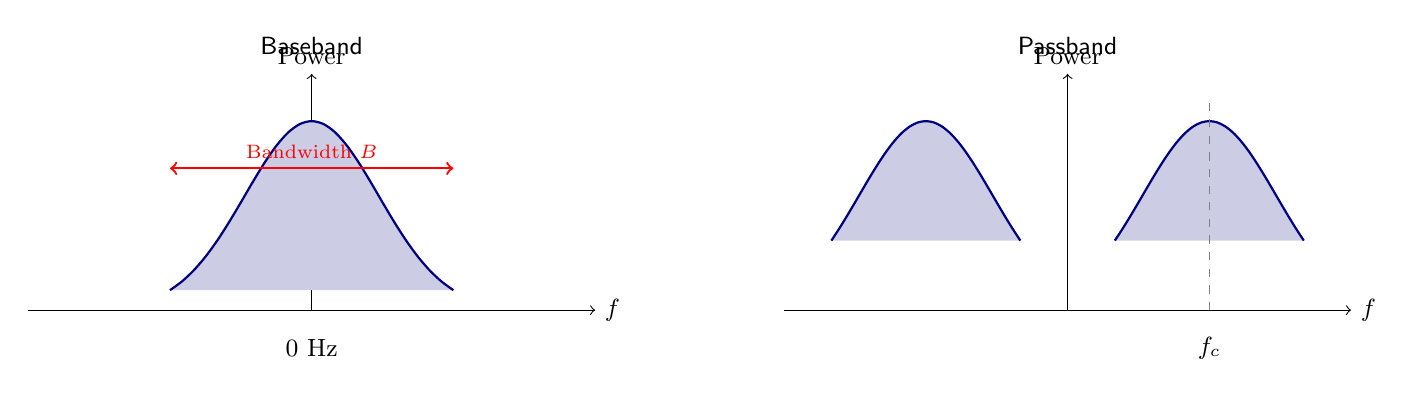
\begin{tikzpicture}[scale=1.2]
% Baseband spectrum
\begin{scope}
\draw[->] (-3,0) -- (3,0) node[right] {\small $f$};
\draw[->] (0,0) -- (0,2.5) node[above] {\small Power};
\draw[thick,NavyBlue,fill=NavyBlue!20] 
  plot[smooth,domain=-1.5:1.5] (\x,{2*exp(-(\x)^2)});
\node at (0,-0.4) {\small 0 Hz};
\node at (0,2.8) {\sffamily\small Baseband};
\draw[<->,red,thick] (-1.5,1.5) -- (1.5,1.5) node[midway,above] {\scriptsize Bandwidth $B$};
\end{scope}

% Passband spectrum
\begin{scope}[xshift=8cm]
\draw[->] (-3,0) -- (3,0) node[right] {\small $f$};
\draw[->] (0,0) -- (0,2.5) node[above] {\small Power};
\draw[thick,NavyBlue,fill=NavyBlue!20] 
  plot[smooth,domain=-2.5:-0.5] (\x,{2*exp(-(\x+1.5)^2)});
\draw[thick,NavyBlue,fill=NavyBlue!20] 
  plot[smooth,domain=0.5:2.5] (\x,{2*exp(-(\x-1.5)^2)});
\draw[dashed,gray] (1.5,0) -- (1.5,2.2);
\node at (1.5,-0.4) {\small $f_c$};
\node at (0,2.8) {\sffamily\small Passband};
\end{scope}
\end{tikzpicture}
\end{center}

\textbf{Key difference:} Baseband processing is simpler (lower sampling rates), while passband transmission enables frequency-division multiplexing and antenna matching. See {[}{[}Baseband-vs-Passband-Signals{]}{]} for detailed coverage.

\subsection{Constellation Diagrams}

A \textbf{constellation diagram} is the complex-plane representation of all possible transmitted symbols in a digital modulation scheme.

\textbf{Mathematical definition:} Each symbol $s_k$ is a point in the complex plane:
\begin{equation}
s_k = I_k + jQ_k = A_k e^{j\theta_k}
\label{eq:constellation}
\end{equation}

where $k \in \{0, 1, \ldots, M-1\}$ for $M$-ary modulation.

\begin{center}
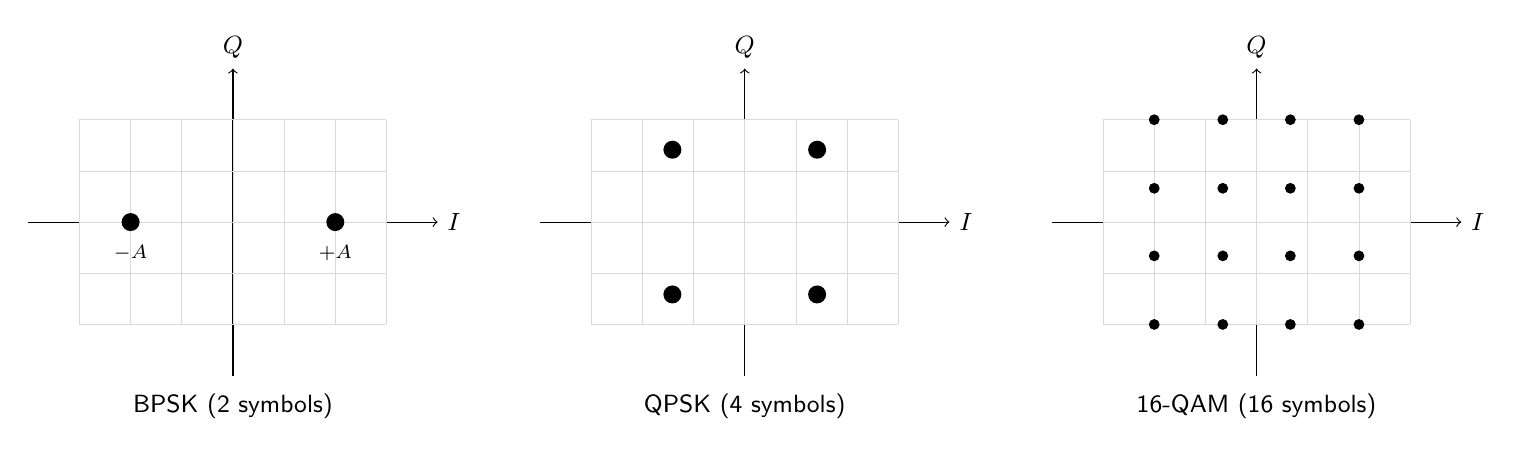
\begin{tikzpicture}[scale=1.3]
% BPSK
\begin{scope}
\draw[->] (-2,0) -- (2,0) node[right] {\small $I$};
\draw[->] (0,-1.5) -- (0,1.5) node[above] {\small $Q$};
\draw[very thin,gray!30] (-1.5,-1) grid[step=0.5] (1.5,1);
\fill[black] (-1,0) circle (2.5pt);
\fill[black] (1,0) circle (2.5pt);
\node[below=5pt] at (-1,0) {\scriptsize $-A$};
\node[below=5pt] at (1,0) {\scriptsize $+A$};
\node at (0,-1.8) {\sffamily\small BPSK (2 symbols)};
\end{scope}

% QPSK
\begin{scope}[xshift=5cm]
\draw[->] (-2,0) -- (2,0) node[right] {\small $I$};
\draw[->] (0,-1.5) -- (0,1.5) node[above] {\small $Q$};
\draw[very thin,gray!30] (-1.5,-1) grid[step=0.5] (1.5,1);
\fill[black] (-0.707,-0.707) circle (2.5pt);
\fill[black] (0.707,-0.707) circle (2.5pt);
\fill[black] (-0.707,0.707) circle (2.5pt);
\fill[black] (0.707,0.707) circle (2.5pt);
\node at (0,-1.8) {\sffamily\small QPSK (4 symbols)};
\end{scope}

% 16-QAM
\begin{scope}[xshift=10cm]
\draw[->] (-2,0) -- (2,0) node[right] {\small $I$};
\draw[->] (0,-1.5) -- (0,1.5) node[above] {\small $Q$};
\draw[very thin,gray!30] (-1.5,-1) grid[step=0.5] (1.5,1);
\foreach \x in {-1,-0.33,0.33,1}
  \foreach \y in {-1,-0.33,0.33,1}
    \fill[black] (\x,\y) circle (1.5pt);
\node at (0,-1.8) {\sffamily\small 16-QAM (16 symbols)};
\end{scope}
\end{tikzpicture}
\end{center}

\begin{calloutbox}{Noise and Decision Regions}
The \textbf{minimum Euclidean distance} $d_{\text{min}}$ between constellation points determines noise immunity:
\begin{equation}
d_{\text{min}} = \min_{i \neq k} |s_i - s_k|
\end{equation}
Larger $d_{\text{min}}$ provides better bit error rate (BER) performance at the expense of higher power or bandwidth.
\end{calloutbox}

See {[}{[}Constellation-Diagrams{]}{]} for detailed analysis and design principles.

\subsection{Symbol Definition and Bit Mapping}

A \textbf{symbol} is the fundamental transmission unit in digital modulation, representing one or more bits encoded as a specific waveform or constellation point.

\textbf{Relationship between bits and symbols:}
\begin{equation}
M = 2^b
\label{eq:symbol_order}
\end{equation}

where:
\begin{itemize}
\item $M$ = number of distinct symbols (modulation order)
\item $b$ = bits per symbol
\end{itemize}

\textbf{Common mappings:}
\begin{center}
\begin{tabular}{lccc}
\toprule
\textbf{Modulation} & \textbf{$M$} & \textbf{Bits/Symbol} & \textbf{Symbol Rate} \\
\midrule
BPSK & 2 & 1 & $R_s = R_b$ \\
QPSK & 4 & 2 & $R_s = R_b/2$ \\
8PSK & 8 & 3 & $R_s = R_b/3$ \\
16-QAM & 16 & 4 & $R_s = R_b/4$ \\
64-QAM & 64 & 6 & $R_s = R_b/6$ \\
256-QAM & 256 & 8 & $R_s = R_b/8$ \\
\bottomrule
\end{tabular}
\end{center}

where $R_b$ is bit rate and $R_s$ is symbol rate.

\begin{keyconcept}
Higher-order modulation ($M > 2$) trades \textbf{spectral efficiency} (more bits per symbol) for \textbf{power efficiency} (symbols closer together, less noise margin). The optimal choice depends on whether your channel is bandwidth-limited or power-limited.
\end{keyconcept}

See {[}{[}What-Are-Symbols{]}{]} for comprehensive coverage.

\subsection{Multipath Fading}

\textbf{Fading} refers to rapid variations in received signal strength caused by constructive and destructive interference of multiple propagation paths.

\textbf{Mathematical model:}
\begin{equation}
r(t) = \sum_{i=1}^{N} \alpha_i e^{j\theta_i} s(t - \tau_i) + n(t)
\label{eq:multipath}
\end{equation}

where:
\begin{itemize}
\item $\alpha_i$ = amplitude of path $i$
\item $\theta_i$ = phase shift of path $i$
\item $\tau_i$ = time delay of path $i$
\item $n(t)$ = additive noise
\end{itemize}

\textbf{Key fading distributions:}

\begin{enumerate}
\item \textbf{Rayleigh fading} (no line-of-sight):
\begin{equation}
p(\alpha) = \frac{\alpha}{\sigma^2} e^{-\alpha^2/(2\sigma^2)}, \quad \alpha \geq 0
\label{eq:rayleigh}
\end{equation}

\item \textbf{Rician fading} (dominant line-of-sight + multipath):
\begin{equation}
p(\alpha) = \frac{\alpha}{\sigma^2} e^{-(\alpha^2 + A^2)/(2\sigma^2)} I_0\left(\frac{\alpha A}{\sigma^2}\right)
\label{eq:rician}
\end{equation}
where $A$ is the amplitude of the line-of-sight component and $I_0$ is the modified Bessel function of the first kind.
\end{enumerate}

\begin{center}
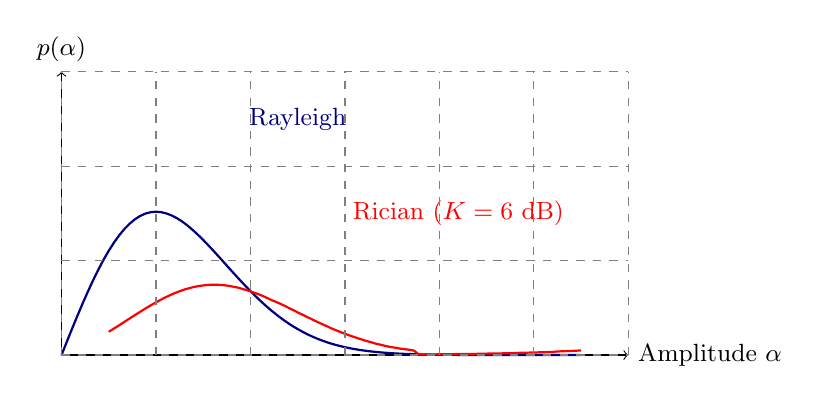
\begin{tikzpicture}[scale=1.2]
\draw[->] (0,0) -- (6,0) node[right] {\small Amplitude $\alpha$};
\draw[->] (0,0) -- (0,3) node[above] {\small $p(\alpha)$};

% Rayleigh
\draw[thick,NavyBlue,domain=0:5.5,samples=100] 
  plot (\x,{2.5*\x*exp(-\x*\x*0.5)});
\node[NavyBlue] at (2.5,2.5) {\small Rayleigh};

% Rician K=6dB
\draw[thick,Red,domain=0.5:5.5,samples=100] 
  plot (\x,{2.5*\x*exp(-0.5*(\x*\x+4))*exp(2*\x*0.5)});
\node[Red] at (4.2,1.5) {\small Rician ($K=6$ dB)};

\draw[dashed,gray] (0,0) grid[step=1] (6,3);
\end{tikzpicture}
\end{center}

\textbf{Mitigation techniques:}
\begin{itemize}
\item \textbf{Diversity} (space, time, frequency)
\item \textbf{Equalization} (removing channel distortion)
\item \textbf{Spread spectrum} (averaging over frequency)
\item \textbf{Interleaving} (distributing burst errors)
\end{itemize}

See {[}{[}Multipath-Propagation-\&-Fading-(Rayleigh,-Rician){]}{]} for detailed coverage.

\subsection{Link Budget Analysis}

A \textbf{link budget} is a systematic accounting of all gains and losses from transmitter to receiver, ensuring sufficient signal-to-noise ratio (SNR) for reliable communication.

\textbf{Fundamental link budget equation:}
\begin{equation}
P_{\text{RX}} = P_{\text{TX}} + G_{\text{TX}} - L_{\text{FSPL}} - L_{\text{atm}} + G_{\text{RX}} - L_{\text{misc}}
\label{eq:link_budget}
\end{equation}

where all values are in dBm or dB:
\begin{itemize}
\item $P_{\text{TX}}$ = Transmit power
\item $G_{\text{TX}}$ = Transmit antenna gain
\item $L_{\text{FSPL}}$ = Free-space path loss
\item $L_{\text{atm}}$ = Atmospheric losses
\item $G_{\text{RX}}$ = Receive antenna gain
\item $L_{\text{misc}}$ = Miscellaneous losses (cables, connectors, etc.)
\end{itemize}

\textbf{Free-space path loss:}
\begin{equation}
L_{\text{FSPL}} = 20\log_{10}(d) + 20\log_{10}(f) + 20\log_{10}\left(\frac{4\pi}{c}\right) \approx 20\log_{10}(d) + 20\log_{10}(f) - 147.55
\label{eq:fspl}
\end{equation}

where:
\begin{itemize}
\item $d$ = distance in meters
\item $f$ = frequency in Hz
\item $c$ = speed of light ($3 \times 10^8$ m/s)
\end{itemize}

Or simplified for practical use:
\begin{equation}
L_{\text{FSPL}}(\text{dB}) = 32.45 + 20\log_{10}(d_{\text{km}}) + 20\log_{10}(f_{\text{MHz}})
\label{eq:fspl_simple}
\end{equation}

See {[}{[}Complete-Link-Budget-Analysis{]}{]} and {[}{[}Free-Space-Path-Loss-(FSPL){]}{]} for detailed coverage.

\subsection{Diversity Techniques}

\textbf{Diversity} exploits multiple independent signal paths to combat fading, dramatically improving reliability without increasing transmit power.

\textbf{Types of diversity:}

\begin{enumerate}
\item \textbf{Space diversity}: Multiple antennas separated by $> \lambda/2$
\begin{equation}
\text{SNR}_{\text{combined}} = \text{SNR}_1 + \text{SNR}_2 + \cdots + \text{SNR}_N \quad \text{(MRC)}
\label{eq:mrc}
\end{equation}

\item \textbf{Frequency diversity}: Transmit same data on multiple carriers separated by $> B_c$ (coherence bandwidth)

\item \textbf{Time diversity}: Transmit same data at different times separated by $> T_c$ (coherence time)

\item \textbf{Polarization diversity}: Use orthogonal polarizations (vertical + horizontal, or LHCP + RHCP)
\end{enumerate}

\begin{calloutbox}{Diversity Gain}
With $N$ independent diversity branches, the probability of deep fade ($< -X$ dB) is reduced by factor $N$:
\begin{equation}
P_{\text{fade,diversity}} \approx [P_{\text{fade,single}}]^N
\end{equation}

For Rayleigh fading, 2-branch diversity provides $\sim$10 dB gain at $10^{-2}$ outage probability.
\end{calloutbox}

\section{Worked Example: Applying Glossary Concepts}

This example demonstrates how to apply multiple glossary concepts in a practical satellite communication link design.

\subsection*{Scenario}
Design a \textbf{QPSK downlink} from a LEO satellite at 550 km altitude to a ground station, achieving BER $< 10^{-6}$.

\subsection*{Given Parameters}
\begin{itemize}
\item Frequency: $f = 2.2$ GHz (S-band)
\item Satellite transmit power: $P_{\text{TX}} = 5$ W = 37 dBm
\item TX antenna gain: $G_{\text{TX}} = 12$ dBi (patch array)
\item Distance: $d = 600$ km (worst case, including elevation angle)
\item RX antenna gain: $G_{\text{RX}} = 25$ dBi (3-meter dish)
\item System noise temperature: $T_{\text{sys}} = 150$ K
\item Data rate: $R_b = 10$ Mbps
\item Required $E_b/N_0$ for QPSK: 10.5 dB (at BER $= 10^{-6}$)
\end{itemize}

\subsection*{Step 1: Calculate Free-Space Path Loss}
Using equation \eqref{eq:fspl_simple}:
\begin{align}
L_{\text{FSPL}} &= 32.45 + 20\log_{10}(600) + 20\log_{10}(2200) \nonumber\\
&= 32.45 + 55.56 + 66.85 \nonumber\\
&= 154.86 \text{ dB}
\end{align}

\subsection*{Step 2: Link Budget (Equation \eqref{eq:link_budget})}
\begin{align}
P_{\text{RX}} &= P_{\text{TX}} + G_{\text{TX}} - L_{\text{FSPL}} + G_{\text{RX}} - L_{\text{misc}} \nonumber\\
&= 37 + 12 - 154.86 + 25 - 2 \nonumber\\
&= -82.86 \text{ dBm}
\end{align}

\subsection*{Step 3: Noise Power}
Noise power in bandwidth $B = R_s = R_b/2 = 5$ MHz (since QPSK has 2 bits/symbol):
\begin{equation}
N_0 = k T_{\text{sys}} = 1.38 \times 10^{-23} \times 150 = 2.07 \times 10^{-21} \text{ W/Hz}
\end{equation}
\begin{equation}
P_{\text{noise}} = N_0 B = 2.07 \times 10^{-21} \times 5 \times 10^6 = 1.035 \times 10^{-14} \text{ W} = -139.85 \text{ dBm}
\end{equation}

\subsection*{Step 4: Calculate SNR and $E_b/N_0$}
\begin{equation}
\text{SNR} = P_{\text{RX}} - P_{\text{noise}} = -82.86 - (-139.85) = 56.99 \text{ dB}
\end{equation}

For QPSK with 2 bits per symbol:
\begin{align}
E_b/N_0 &= \text{SNR} - 10\log_{10}(R_b/B) \nonumber\\
&= 56.99 - 10\log_{10}(10/5) \nonumber\\
&= 56.99 - 3.01 = 53.98 \text{ dB}
\end{align}

\subsection*{Step 5: Link Margin}
\begin{equation}
\text{Margin} = (E_b/N_0)_{\text{actual}} - (E_b/N_0)_{\text{required}} = 53.98 - 10.5 = 43.48 \text{ dB}
\end{equation}

\begin{keyconcept}
\textbf{Excellent link margin!} The 43.5 dB margin provides substantial protection against:
\begin{itemize}
\item Atmospheric attenuation (rain, clouds): $\sim$2--5 dB
\item Multipath fading: $\sim$10--20 dB (can use diversity)
\item Polarization mismatch: $\sim$3 dB
\item Implementation losses: $\sim$2--3 dB
\item Link availability target: 99.9\% even in adverse conditions
\end{itemize}
\end{keyconcept}

\subsection*{Key Concepts Applied}
This example integrated multiple glossary concepts:
\begin{itemize}
\item \textbf{QPSK modulation}: 2 bits/symbol (see \S\ref{sec:key-concepts})
\item \textbf{Link budget}: Equation \eqref{eq:link_budget}
\item \textbf{Free-space path loss}: Equation \eqref{eq:fspl_simple}
\item \textbf{$E_b/N_0$}: Energy per bit to noise ratio
\item \textbf{SNR}: Signal-to-noise ratio
\item \textbf{Fading margin}: Protection against multipath
\end{itemize}

\section{Applications and Usage Guide}

This glossary serves multiple purposes for different audiences:

\subsection{For Students}
\begin{itemize}
\item \textbf{Quick reference} during problem-solving
\item \textbf{Equation lookup} for homework and exams
\item \textbf{Concept review} before chapter reading
\item \textbf{Cross-referencing} to find related topics
\end{itemize}

\subsection{For Practitioners}
\begin{itemize}
\item \textbf{System design} parameter reference
\item \textbf{Link budget} calculations (equations \eqref{eq:link_budget}--\eqref{eq:fspl_simple})
\item \textbf{Modulation selection} guidance (constellation diagrams)
\item \textbf{Performance estimation} (BER, SNR relationships)
\end{itemize}

\subsection{For Researchers}
\begin{itemize}
\item \textbf{Notation standardization} across publications
\item \textbf{Quick concept verification}
\item \textbf{Literature cross-reference} to detailed chapters
\item \textbf{Teaching resource} for courses and tutorials
\end{itemize}

\begin{calloutbox}{Digital Navigation}
\textbf{Using this glossary effectively:}
\begin{enumerate}
\item Use PDF search (Ctrl+F / Cmd+F) to find terms instantly
\item Follow {[}{[}Chapter-Name{]}{]} links for detailed coverage
\item Check equation numbers for cross-referencing
\item Use Section \ref{sec:key-concepts} for conceptual deep-dives
\item Refer to worked example for integrated application
\end{enumerate}
\end{calloutbox}

\section{Summary}

This glossary provides:
\begin{itemize}
\item \textbf{191 acronyms and abbreviations} organized alphabetically (Sections \ref{a}--\ref{z})
\item \textbf{Detailed explanations} of 7 fundamental concepts with equations and diagrams
\item \textbf{TikZ visual aids}: constellation diagrams, spectrum plots, fading distributions
\item \textbf{13 numbered equations} for quantitative analysis
\item \textbf{Worked example} integrating multiple concepts in satellite link design
\item \textbf{Cross-references} to 30+ detailed chapters
\end{itemize}

\begin{keyconcept}
\textbf{This glossary is a living reference.} As you progress through the book, return here to refresh your understanding, verify notation, and explore connections between concepts. The cross-references create a knowledge graph linking all 69 chapters.
\end{keyconcept}

\vspace{1em}
\noindent\emph{For detailed explanations of any term, follow the chapter cross-references or use the book index.}

\vspace{0.5em}
\noindent\emph{Last updated: October 2025}
